%% LyX 1.3 created this file.  For more info, see http://www.lyx.org/.
%% Do not edit unless you really know what you are doing.
\documentclass[english]{article}
\usepackage[T1]{fontenc}
\usepackage[latin1]{inputenc}
\usepackage{graphicx}

\makeatletter
%%%%%%%%%%%%%%%%%%%%%%%%%%%%%% User specified LaTeX commands.

\usepackage{babel}
\makeatother
\begin{document}

\author{thomas.leibovici@cea.fr}
\title{\center{ \Large \textbf{Exporting GANESHA's statistics with SNMP} }}
\maketitle

%% \tableofcontents
%% \newpage

GANESHA is able to export its internal statistics so that an administrator can browse them using the SNMP protocol.
It also provides a client for easily broswing its SNMP tree in a convivial and human understandable way.

This document describes the requirements for this feature (libraries needed,
SNMPd configuration...) and how to enable and configure it in GANESHA NFSD.

\section{Requirements}

SNMP support in GANESHA is based on the Net-SNMP library. This is a free implementation
of SNMP that comes with most Linux distributions. It can also be retrieved from \texttt{http://net-snmp.sourceforge.net}.

GANESHA's SNMP support has been validated with Net-SNMP v5.1.4. However, Net-SNMP v5.4 or higher is recommended.

Install the following packages on the machine where you are compiling and running GANESHA NFSD:

\begin{itemize}
\item \emph{net-snmp} contains the snmpd and snmptrapd daemons ;
\item \emph{net-snmp-utils} contains various utilities for snmp ;
\item \emph{net-snmp-perl} contains the perl API ;
\item \emph{net-snmp-devel} contains the development libraries and
header files.
\end{itemize}

Note that the net-snmp library needs symbols defined in \emph{lm-sensors} and \emph{openssl} libraries,
so you will also need to install \emph{lm-sensors-devel} and \emph{openssl-devel} packages on your system.

\medskip
For using the SNMP client tool \texttt{snmp\_adm} provided with GANESHA, you will also need the following perl modules:

\begin{itemize}
\item
  \emph{SNMP}\footnote{\texttt{http://search.cpan.org/~gsm/SNMP-5.0400001/SNMP.pm}}
  provided by the \emph{net-snmp-perl} RedHat's package
\item \emph{XML::DOM}\footnote{\texttt{http://search.cpan.org/~tjmather/XML-DOM-1.44/lib/XML/DOM.pm}}
  for XML outputs.
  \item
  \emph{Getopt::Std}\footnote{\texttt{http://search.cpan.org/~nwclark/perl-5.8.8/lib/Getopt/Std.pm}}
  to parse command line options.
  \item \emph{Config::General}\footnote{\texttt{http://search.cpan.org/~tlinden/Config-General-2.33/General.pm}}
 to parse config file
\item
  \emph{SNMP::Trapinfo}\footnote{\texttt{http://search.cpan.org/~tonvoon/SNMP-Trapinfo-1.0/lib/SNMP/Trapinfo.pm}}
  to manage SNMP traps.
\end{itemize}


\section{SNMPd setup}

GANESHA does not handle SNMP requests directly. Actually, it registers its SNMP sub-tree
on a SNMPd daemon, using an extention of the SNMP protocol called \emph{AgentX}.

The SNMPd daemon that exports GANESHA's SNMP tree can be located on the same host,
but it can also run on a remote management station.

\medskip
For activating agentX extension, add the following line
to your SNMPd configuration file (default location is \texttt{/etc/snmp/snmpd.conf}):
\begin{verbatim}
master agentx
\end{verbatim}

You must then specify a way to communicate with GANESHA:
\begin{itemize}
\item if it runs on the same host, you can use a socket file.
In this case, add the following line to SNMPd configuration file \texttt{/etc/snmp/snmpd.conf}:
\begin{verbatim}
AgentXSocket <path to the socket file>

E.g:
AgentXSocket /var/tmp/agentx/sock_file
\end{verbatim}
\item In any case (local or remote SNMPd), you can also use a standard
socket connection:
\begin{verbatim}
AgentXSocket <protocol>[:<network interface address>]:<port number>

E.g:
# listening on a single network interface
AgentXSocket tcp:192.168.0.42:761

# listening on all network interfaces
AgentXSocket tcp:761
\end{verbatim}

Note that the AgentX default port number is 705.
\end{itemize}

\medskip
Your SNMPd is now ready for exporting GANESHA statistics.
Restart it after you changed its configuration file.

\medskip
Note: if you want to restrict the access of GANESHA's SNMP subtree,
refer to the snmpd documentation about \emph{views}, \emph{groups},
\emph{SNMPv2 communities}, and \emph{SNMPv3 authentication}.


\section{Enabling SNMP support in GANESHA}

\subsection{Compilation}

By default, GANESHA is compiled without SNMP support.
To enable this feature, add \texttt{--enable-snmp-adm} argument
to the \texttt{configure} command line.

\begin{verbatim}
E.g:
./configure --with-fsal=FUSE --enable-snmp-adm
\end{verbatim}

\subsection{Configuration}

A specific section of GANESHA's configuration file is dedicated
to SNMP options.
This block must be labelized with the \texttt{SNMP\_ADM} tag.

It must include the following parameters:

\begin{itemize}
\item \textbf{snmp\_agentx\_socket}: the socket file or the network interface
for communicating with SNMPd (as it appears in the SNMPd configuration file).
\item \textbf{product\_id}: this number must be unique for each instance of GANESHA
you are exporting with the same SNMPd.
\item \textbf{snmp\_adm\_log}: The log file for SNMP related logs.

\item \textbf{export\_cache\_stats}: indicates if cache stats are exported.
\item \textbf{export\_requests\_stats}: indicates if NFS requests stats are exported.
\item \textbf{export\_maps\_stats}: indicates if UID/GID map stats are exported.
\item \textbf{export\_buddy\_stats}: indicates if memory usage stats are exported.

\item \textbf{export\_nfs\_calls\_detail}: indicates if detailled stats about NFS calls are exported.
\item \textbf{export\_cache\_inode\_calls\_detail}: indicates if detailled stats about metadata cache calls are exported.
\item \textbf{export\_fsal\_calls\_detail}: indicates if detailled stats about filesystem calls are exported.
\end{itemize}


\begin{verbatim}
E.g:

SNMP_ADM
{
    snmp_agentx_socket = "tcp:localhost:761";
    product_id = 2;
    snmp_adm_log = "/var/log/ganesha/snmp_adm.log";

    export_cache_stats    = TRUE;
    export_requests_stats = TRUE;
    export_maps_stats     = FALSE;
    export_buddy_stats    = TRUE;

    export_nfs_calls_detail = FALSE;
    export_cache_inode_calls_detail = FALSE;
    export_fsal_calls_detail = FALSE;
}
\end{verbatim}


\section{Browsing GANESHA's SNMP tree}

\subsection{Tree description}

The SNMP tree of GANESHA is located under this OID:
\begin{verbatim}
.iso.org.dod.internet.private.enterprise.cea.snmp-admin.<product_id>
\end{verbatim}
where \texttt{product\_id} is the value you specified in GANESHA's config file.
If some MIBs are missing, you can however access the tree with the numeric OID:
\begin{verbatim}
.1.3.6.1.4.1.12384.999.<product_id>
\end{verbatim}

\medskip

The product subtree is planned to be divided in tree parts:
\begin{itemize}
\item \texttt{<product\_root>.0} contains dynamic statistics of the NFSD;
\item \texttt{<product\_root>.1} contains configuration values;
\item \texttt{<product\_root>.2} contains special OIDs for executing administrative
actions on the daemon (flushing cache, ...).
\end{itemize}

At this time, only the first subtree (\texttt{<product\_root>.0}) is exported.

\medskip

GANESHA's SNMP tree is self-descriptive and it can be understood without any
specific MIB installed on your system.

Thus, each exported value \texttt{<i>} is described by the following OIDs:

\begin{itemize}
\item \texttt{<product\_root>.0.<i>.0} contains the name of the variable
\item \texttt{<product\_root>.0.<i>.1} contains the description of it
\item \texttt{<product\_root>.0.<i>.2.0} is the type of the variable\footnote{This is mainly unsed
for handling 64 bits integers. Indeed, as SNMP doesn't support them, we return them
as a string but this field will indicate they must be interpreted as integers.}.
\item \texttt{<product\_root>.0.<i>.2.1} contains the value.
\end{itemize}

This tree is represented in the figure \ref{figtree}.

\begin{figure}
  \center 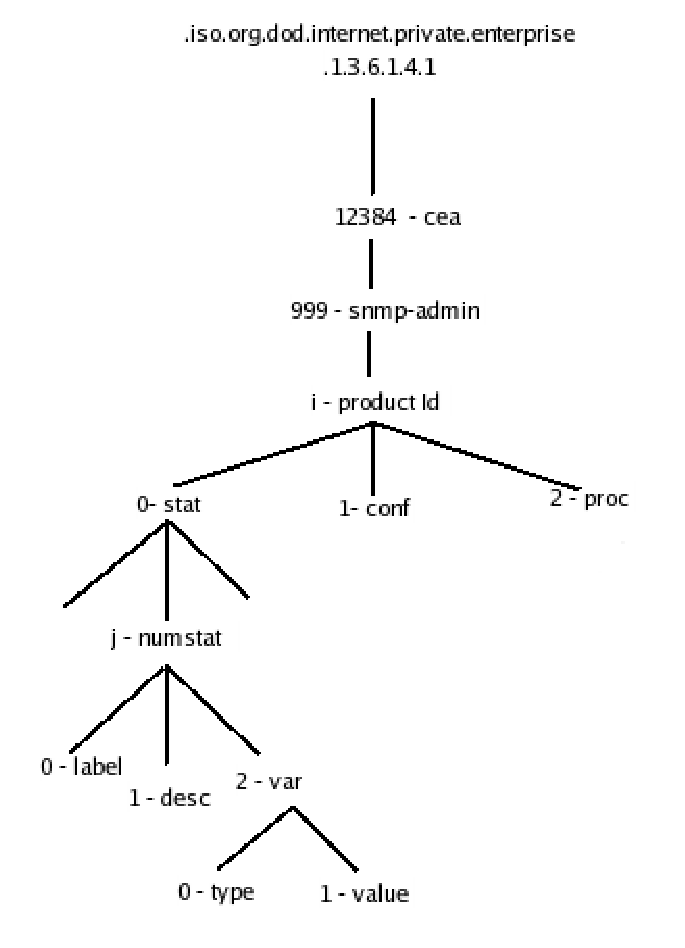
\includegraphics[scale=0.6]{snmp_tree.eps}
  \caption{GANESHA's SNMP tree}
  \label{figtree}
\end{figure}

\medskip

Example of \texttt{snmp\_walk} on a GANESHA variable:

\begin{verbatim}
> snmpwalk -v 2c -c public localhost  .1.3.6.1.4.1.12384.999.2.0.4
SNMPv2-SMI::enterprises.12384.999.2.0.4.0 = STRING: "cache_nb_entries"
SNMPv2-SMI::enterprises.12384.999.2.0.4.1 = STRING: "number of entries in cache"
SNMPv2-SMI::enterprises.12384.999.2.0.4.2.0 = STRING: "INTEGER"
SNMPv2-SMI::enterprises.12384.999.2.0.4.2.1 = INTEGER: 51
\end{verbatim}


\subsection{Using the SNMP client provided with GANESHA}

Even if GANESHA statistics can be browsed using standard SNMP commands
(\texttt{snmp\_get}, \texttt{snmp\_walk}...), GANESHA comes with a SNMP client tool
(\texttt{snmp\_adm})
for easily browsing those stats in a convivial way, without having to handle OIDs,
and all SNMP relative stuff.

It is located in the '\texttt{snmp\_adm/client}' directory of GANESHA's distribution,
and is also available in GANESHA RPMs that include SNMP support.

\subsubsection{\texttt{snmp\_adm} client configuration file}

If you're bored of typing OIDs, SNMP version, community name and all that stuff,
just create a \texttt{.snmp\_adm.conf} file in your home (with mode 600) with the following
lines inside:
\begin{verbatim}
host       <snmpd_address>[:<snmpd_port>]
product_id <the product id of your favorite NFS server>

#if you are using SNMPv3 protocol, also specify the following information:
# password for authentication
auth_pass "password"
# password for encoding
enc_pass "password"
# user name
sec_name "snmpadm"
\end{verbatim}

\subsubsection{SNMP relative options}

If you don't want to use a configuration file,
or if you want to overwrite the values it specifies,
you can indicate them on \texttt{snmp\_adm} command line:
\begin{verbatim}
SNMP relative options:

  -s <host>[:port] : the host where SNMP server is running
      (default is localhost)
  -p <product_id|product_name> : the deamon to be queried
      (default is the first product of server's admin tree)
  -C <community>: Community name for SNMPv2c (default is public).
  -A <auth>: authentication for SNMPv3.
  -X <pass>: password for SNMPv3.
  -u <secname>: security name for SNMPv3.
  -f <path>: path to the configuration file.
\end{verbatim}

\subsubsection{\texttt{snmp\_adm} commands}

The main command you will use is '\texttt{snmp\_adm liststat}'.
When used without options, it only displays the list of available variables.
When used with '\texttt{-d}' it displays the description of each variable.
When used with '\texttt{-v}' it displays the values of variables.
You can also specify an expression, so only the variables
whose name contains this expression will be displayed.

\begin{verbatim}
E.g:

> ./snmp_adm -v liststat cache

Statistics for product_id=2:
name                          type       value

cache_nb_gc_lru_active         INTEGER    176
cache_nb_gc_lru_total          INTEGER    432
cache_nb_call_total            INTEGER    25323
cache_nb_entries               INTEGER    5176
cache_min_rbt_num_node         INTEGER    32
cache_max_rbt_num_node         INTEGER    37
cache_avg_rbt_num_node         INTEGER    34
cache_nbset                    INTEGER    5465
cache_nbtest                   INTEGER    0
cache_nbget                    INTEGER    6243
cache_nbdel                    INTEGER    132
\end{verbatim}



\end{document}


